
\begin{figure}
	\begin{center}
		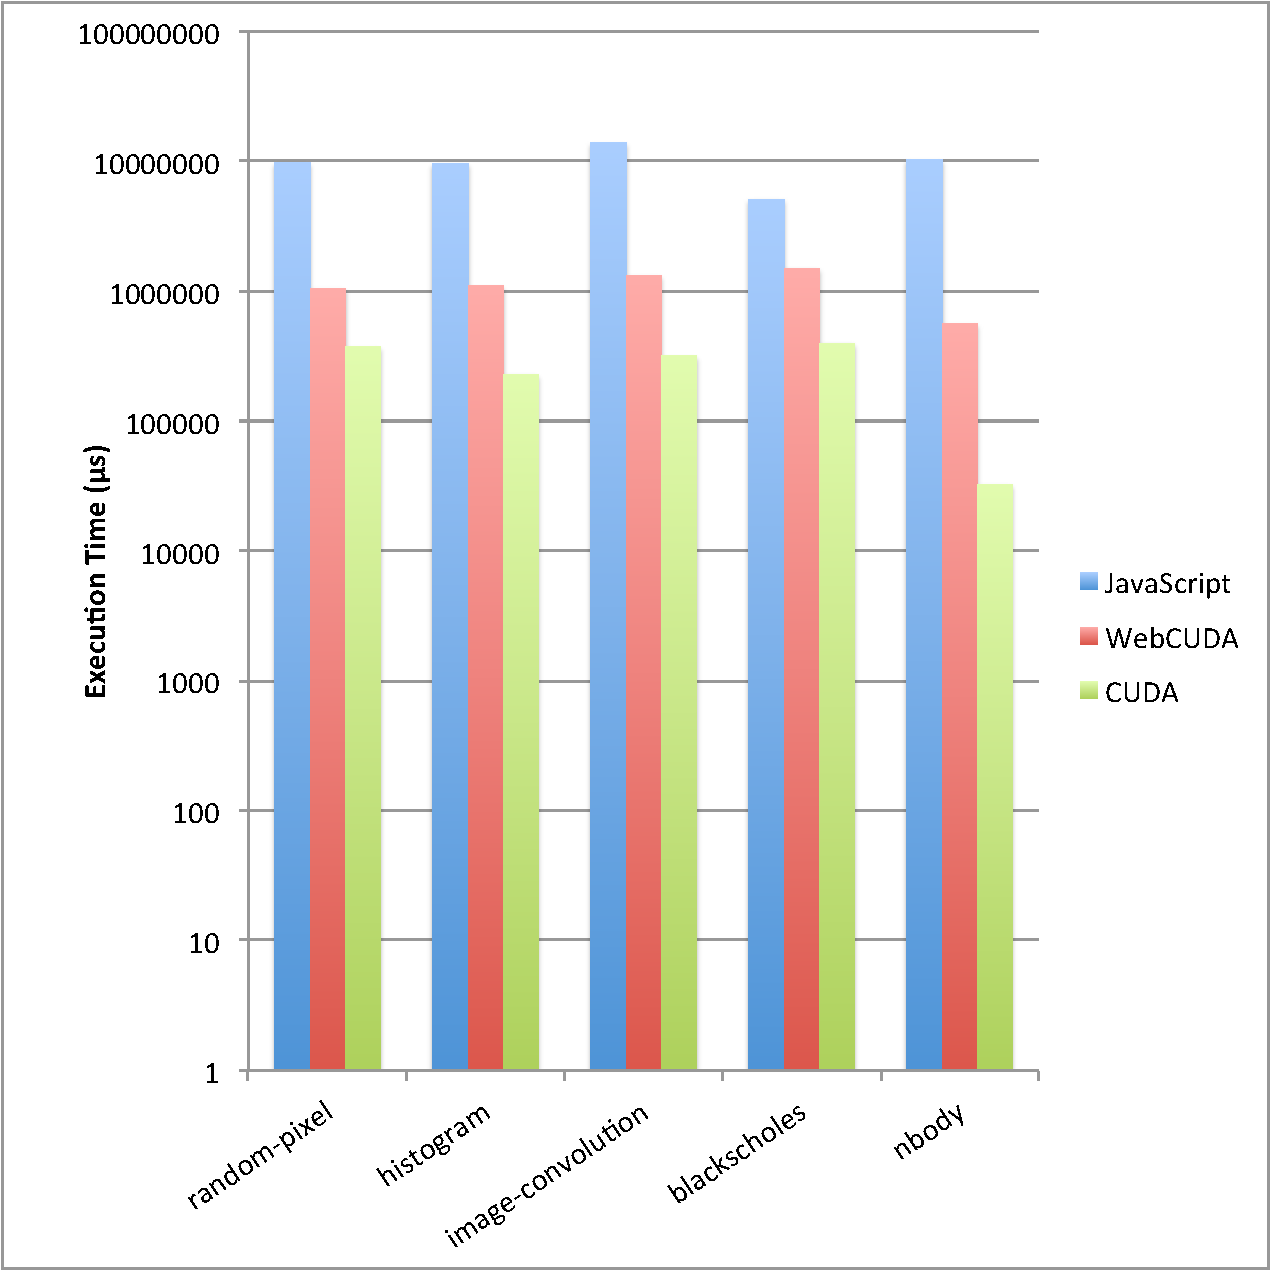
\includegraphics[width=\columnwidth]{./figures/fig1}
	\end{center}
	\caption{Comparison of Execution Time between JavaScript, \namens, and CUDA benchmarks}
	\label{fig1}
\end{figure}

\begin{figure}
	\begin{center}
		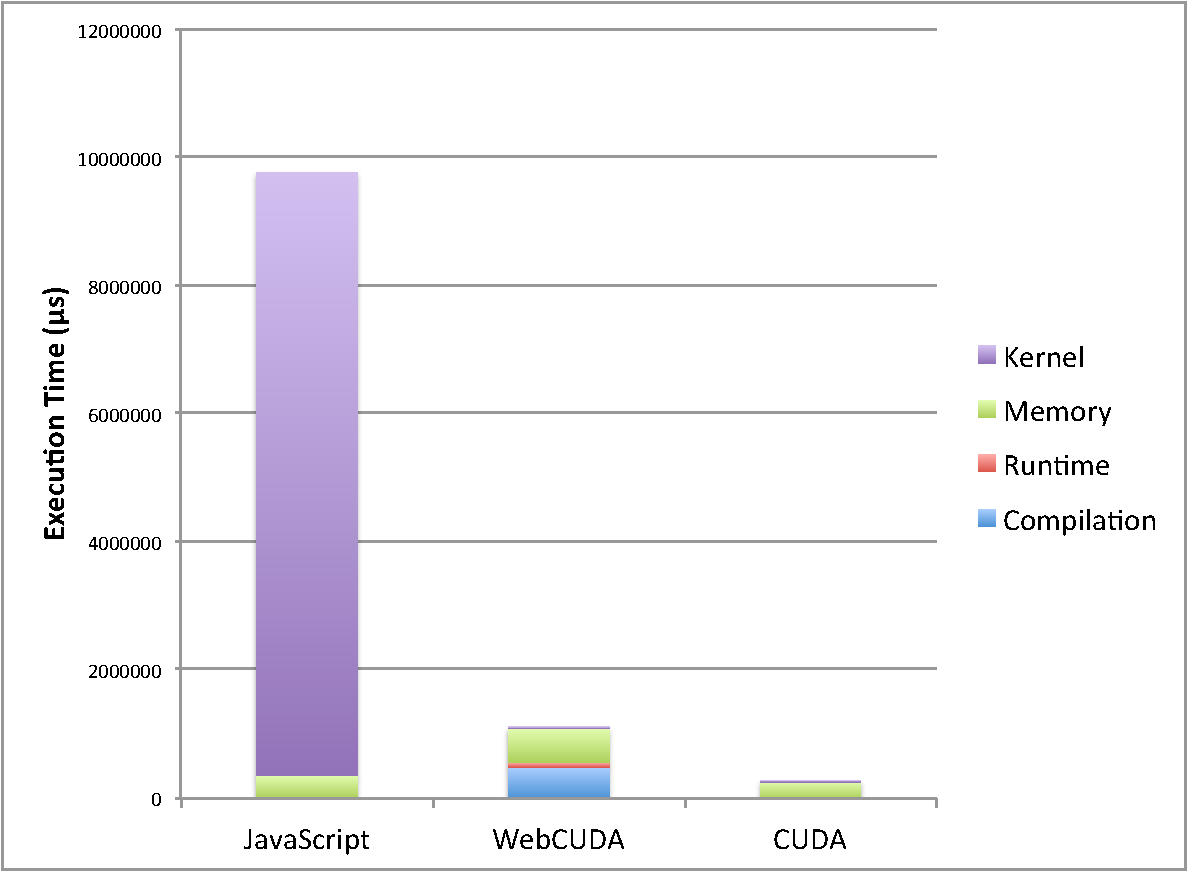
\includegraphics[width=\columnwidth]{./figures/fig2}
	\end{center}
	\caption{Breakdown of Stages of Execution}
	\label{fig2}
\end{figure}

\begin{figure}
	\begin{center}
		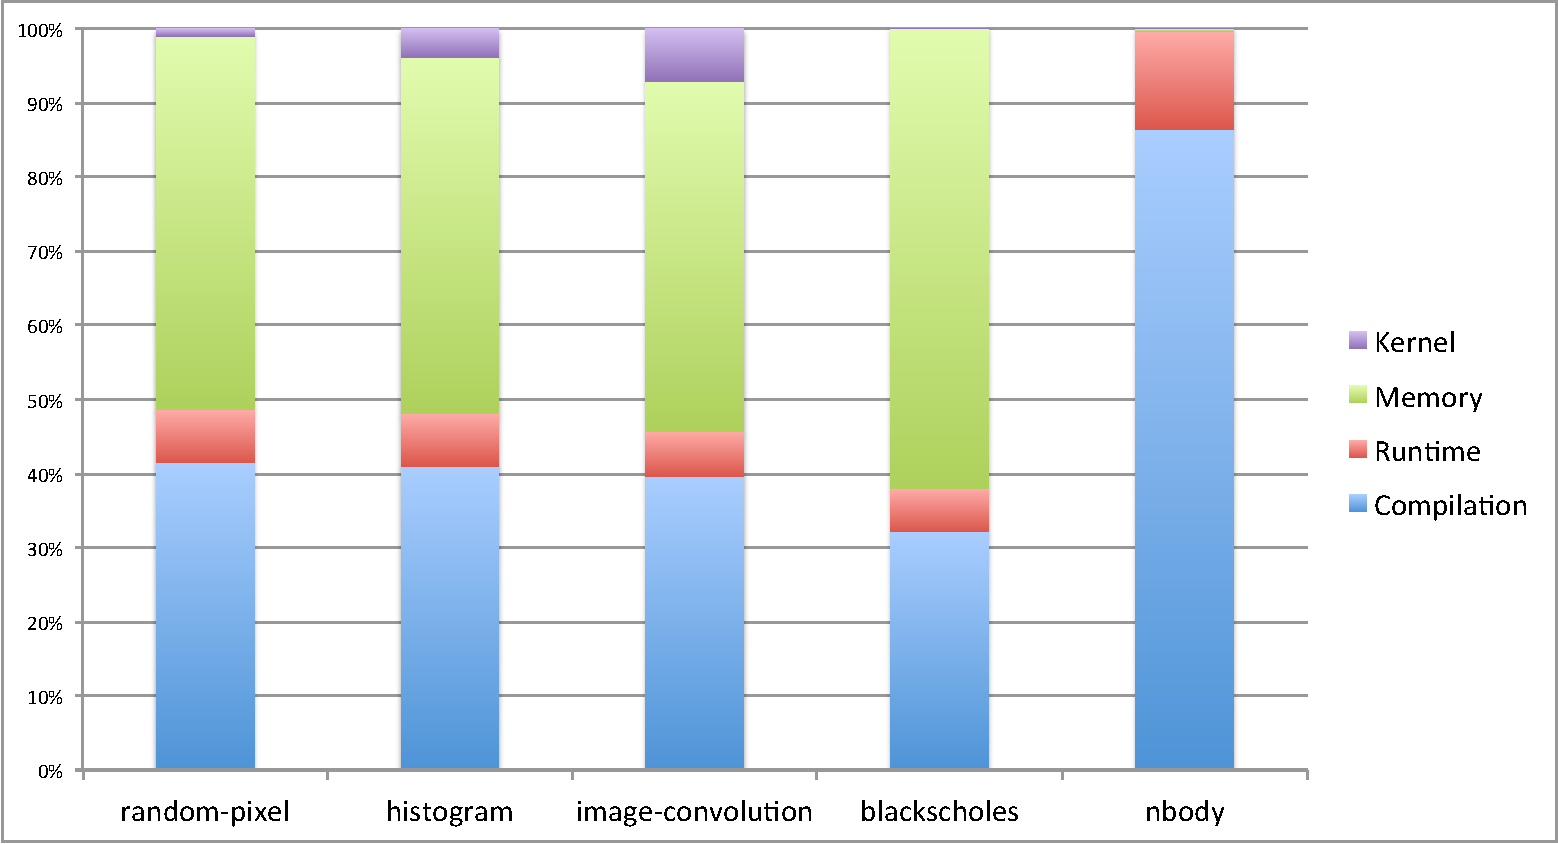
\includegraphics[width=\columnwidth]{./figures/fig3}
	\end{center}
	\caption{Breakdown of Stage of Execution for each \name Benchmark}
	\label{fig3}
\end{figure}

\begin{figure} \begin{center}
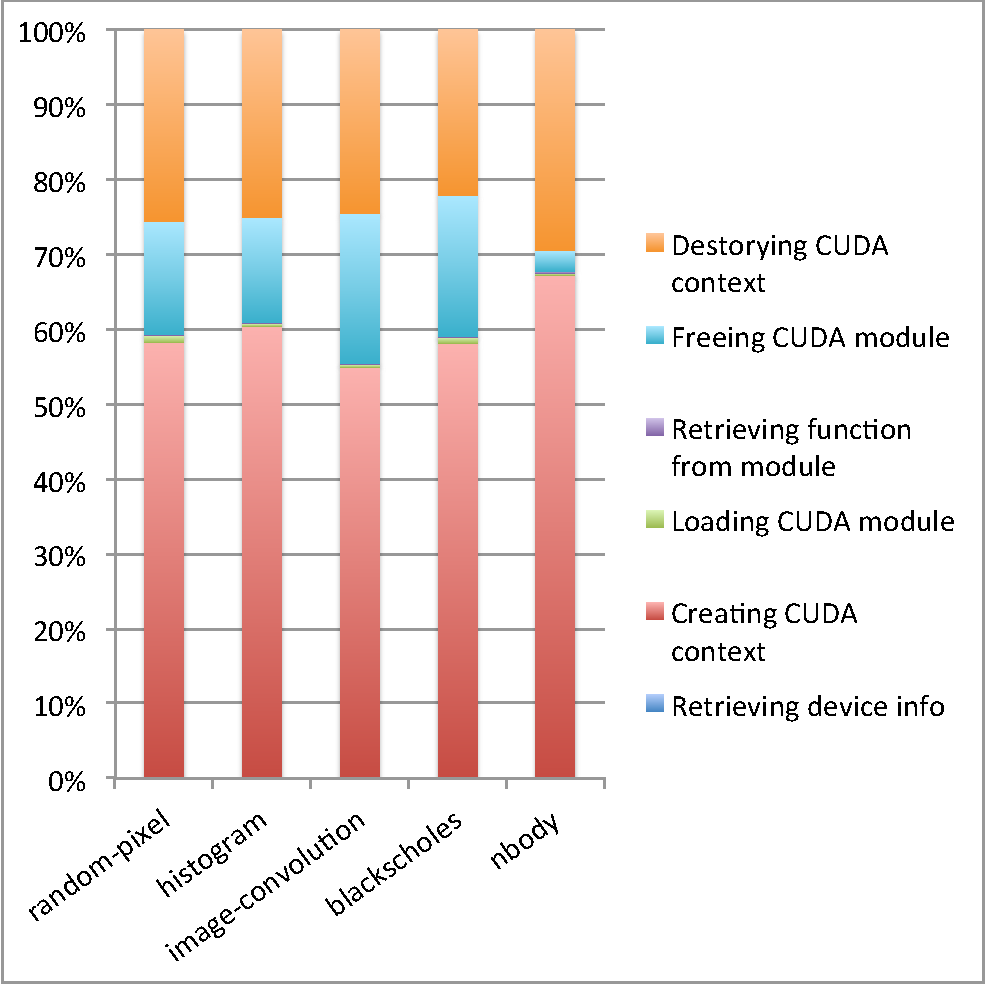
\includegraphics[width=\columnwidth]{./figures/fig4} \end{center}
\caption{Breakdown of Runtime Overhead of \namens} \label{fig4} \end{figure} 


We evaluate our \name implementation against the original V8 JavaScript
engine, which serves as a baseline, and the CUDA framework, which is set as a
reference.

\subsection{Benchmarks}
\begin{table}
	\begin{center}
		\begin{tabular}{| l | l |}
			\hline
			Benchname & Input/Output Size \\
			\hline
			random-pixel & 32M pixel image \\
			\hline
			histogram & 512M elements \\
			\hline
			image-convolution & 16M pixel image \\
			\hline
			blackscholes & 40M options \\
			\hline
			nbody-simulation & 1024 bodies \\
			\hline
		\end{tabular}
	\end{center}
	\caption{Description of Benchmarks use for evaluation.}
	\label{benchmark-table}
\end{table}

To evaluate performance on different platforms, we create different versions of
benchmarks for each domain. We chose 5 CUDA examples, mostly from CUDA SDK
samples, and manually ported them to the \name and JavaScript environments.
Porting to \name versions starts from CUDA versions, and involves rewriting CPU
portions in JavaScript with \name extension and placing CUDA portions in a
separate file. Porting to JavaScript versions is more straightforward, since it
involves translating C code into JavaScript code, which has C-like semantics
for many arithmetic operations.  The input sizes are adjusted as shown in Table
2 to make the amount of computation and the execution time of the JavaScript
benchmark versions nontrivial.

\subsection{Experimental Setup} We run all experiments on the Amazon EC2
\cite{amazonEC2} g2.2xlarge instance to ensure an isolated execution
environment. The g2.2xlarge instance has an Intel Xeon 8-core processor running
at 2.6 GHz and a NVIDIA GRID K520 processor based on the Kepler architecture.
The CUDA driver and runtime version is set to 5.5, which was the most recent
version when the project was started. We use a unmodified version of V8 to run JavaScript benchmarks, a \name-enabled version of V8 to run \name benchmarks, and the NVIDIA CUDA Compiler (nvcc~\cite{nvcc}) to build CUDA benchmarks.

%We build our \namens-enabled
%JavaScript V8 shell on the instance to execute JavaScript and \name benchmarks,
%and we build CUDA benchmarks using NVIDIA CUDA Compiler.

\subsection{Results}

\paragraph{Comparison with JavaScript} Figure~\ref{fig4} shows that \name is
about an order of magnitude faster than JavaScript; on average, it achieves 9x
speedup over JavaScript. As shown in Figure~\ref{fig5}, while computation
consumes the major portion of execution time for JavaScript benchmarks, it is
negligible in \name and CUDA benchmarks thanks to the parallel
nature of the benchmarks and the utilization of a CUDA device optimized for such
parallel computation. \name introduces compilation and runtime overhead to make
use of the CUDA device and some memory overhead for CUDA memory allocation and data
transfer between CPU and CUDA device, but the huge gain from the computation
more than justifies such overheads.

\paragraph{Comparison with CUDA} Compared to CUDA benchmarks, however, \name
still experiences 5x slowdown on average. It is mainly due to two reasons.
First, \name has runtime and compilation overheads which are not present in CUDA.
Second, memory allocation on CPU takes much more time on \namens. \name
allocates CPU memory using JavaScript Typed Array functions while CUDA
allocates CPU memory directly through malloc calls. We suspect that this level of
indirection for memory allocation in JavaScript is a source of slowdown
and leave it as a future work to analyze memory performance between JavaScript
and CUDA.

\paragraph{Compilation Overhead} Figure~\ref{fig6} shows that compilation
overhead is significant and takes up 48\% of the total execution time for \name
benchmarks. This is the time taken to translate a .cu file, which contains source code
written in CUDA, into a .ptx file, which contains an intermediate
representation the CUDA-enabled graphics driver can then execute. \name provides a mean to
load a .ptx file or a .cubin file instead which removes most
compilation overhead and leads to extra 2x (18x overall) speedup over the native JavaScript. A
developer may choose to load a .ptx file for better performance at the cost of
extra maintenance effort of compiling a .cu file offline. In addition, as a .ptx
file is difficult to read without knowledge of intermediate representation, it
will degrade readability and reusability of source code, which is one of the main
benefits of web applications.

\paragraph{V8 Runtime Overhead} Runtime overhead is introduced by \name
takes 7.9\% on average of the total execution time for \name
benchmarks. As shown in Figure~\ref{fig7}, managing the CUDA execution context is
responsible for most of the overhead.

\paragraph{Running Native JavaScript Programs} To verify that the \name
extension does not negatively affect native JavaScript programs, we ran Octane
Benchmark Suite on the original V8 and our \namens-enabled V8 . The Octane
Benchmark Suite~\cite{octane} is a popular JavaScript benchmark suite
consisting of 17 programs, ranging from traditional scientific benchmarks to
realistic web applications, and reports test scores based on the execution
time. We ran it multiple times on the original and modified V8 versions, and
found the test scores to be the same for each version. 


